\documentclass[final]{hcmuitthesis}

% ==========================================================
% 1. CẤU HÌNH GÓI LỆNH (PACKAGES) TỪ FILE CŨ CỦA BẠN
% ==========================================================
\usepackage{graphicx}
\usepackage{listings}
\usepackage[table]{xcolor}
\usepackage{colortbl}
\usepackage[hidelinks]{hyperref}
\usepackage{bookmark}
\usepackage{float}
\usepackage{array}
\usepackage{tikz}
\usetikzlibrary{calc,shapes.geometric,arrows.meta,positioning}

% Định nghĩa màu sắc
\definecolor{codegreen}{rgb}{0,0.6,0}
\definecolor{codegray}{rgb}{0.5,0.5,0.5}
\definecolor{codepurple}{rgb}{0.58,0,0.82}
\definecolor{wordblue}{RGB}{0,112,192}

% Định nghĩa ngôn ngữ TOML và YAML
\lstdefinelanguage{toml}{
  keywords={true,false},
  sensitive=true,
  comment=[l]{\#},
  morestring=[b]"
}
\lstdefinelanguage{yaml}{
  keywords={true,false,null},
  sensitive=true,
  comment=[l]{\#},
  morestring=[b]",
  morestring=[b]'
}

% Cấu hình Listings (Hỗ trợ tiếng Việt và màu sắc)
\lstset{
  backgroundcolor=\color{white},
  basicstyle=\ttfamily\color{black}\footnotesize,
  breaklines=true,
  frame=single,
  rulecolor=\color{black},
  keywordstyle=\color{blue},
  commentstyle=\color{codegreen},
  stringstyle=\color{red},
  numberstyle=\tiny\color{codegray},
  numbers=left,
  showstringspaces=false,
  tabsize=2,
  inputencoding=utf8,
  extendedchars=true,
  escapeinside={\%*}{*)},
  literate=
  {á}{{\'a}}1 {à}{{\`a}}1 {ả}{{\'a}}1 {ã}{{\~a}}1 {ạ}{{\d{a}}}1
  {ă}{{\u{a}}}1 {ắ}{{\'{\u{a}}}}1 {ằ}{{\`{\u{a}}}}1 {ẳ}{{\'{\u{a}}}}1 {ẵ}{{\~{\u{a}}}}1 {ặ}{{\d{\u{a}}}}1
  {â}{{\^{a}}}1 {ấ}{{\'{\^{a}}}}1 {ầ}{{\`{\^{a}}}}1 {ẩ}{{\'{\^{a}}}}1 {ẫ}{{\~{\^{a}}}}1 {ậ}{{\d{\^{a}}}}1
  {đ}{{\dj}}1 {Đ}{{\DJ}}1
  {é}{{\'e}}1 {è}{{\`e}}1 {ẻ}{{\'e}}1 {ẽ}{{\~e}}1 {ẹ}{{\d{e}}}1
  {ê}{{\^{e}}}1 {ế}{{\'{\^{e}}}}1 {ề}{{\`{\^{e}}}}1 {ể}{{\'{\^{e}}}}1 {ễ}{{\~{\^{e}}}}1 {ệ}{{\d{\^{e}}}}1
  {í}{{\'i}}1 {ì}{{\`i}}1 {ỉ}{{\'i}}1 {ĩ}{{\~i}}1 {ị}{{\d{i}}}1
  {ó}{{\'o}}1 {ò}{{\`o}}1 {ỏ}{{\'o}}1 {õ}{{\~o}}1 {ọ}{{\d{o}}}1
  {ô}{{\^{o}}}1 {ố}{{\'{\^{o}}}}1 {ồ}{{\`{\^{o}}}}1 {ổ}{{\'{\^{o}}}}1 {ỗ}{{\~{\^{o}}}}1 {ộ}{{\d{\^{o}}}}1
  {ơ}{{\"o}}1 {ớ}{{\'{\"o}}}1 {ờ}{{\`{\"o}}}1 {ở}{{\'{\"o}}}1 {ỡ}{{\~{\"o}}}1 {ợ}{{\d{\"o}}}1
  {ú}{{\'u}}1 {ù}{{\`u}}1 {ủ}{{\'u}}1 {ũ}{{\~u}}1 {ụ}{{\d{u}}}1
  {ư}{{\"u}}1 {ứ}{{\'{\"u}}}1 {ừ}{{\`{\"u}}}1 {ử}{{\'{\"u}}}1 {ữ}{{\~{\"u}}}1 {ự}{{\d{\"u}}}1
  {ý}{{\'y}}1 {ỳ}{{\`y}}1 {ỷ}{{\'y}}1 {ỹ}{{\~y}}1 {ỵ}{{\d{y}}}1
}

% ==========================================================
% 2. KHAI BÁO METADATA (THÔNG TIN ĐỒ ÁN)
% ==========================================================
\upperuniname{ĐẠI HỌC QUỐC GIA THÀNH PHỐ HỒ CHÍ MINH}
\uniname{TRƯỜNG ĐẠI HỌC CÔNG NGHỆ THÔNG TIN}
\deptname{KHOA MẠNG MÁY TÍNH VÀ TRUYỀN THÔNG}
\stumajor{KỸ SƯ NGÀNH AN TOÀN THÔNG TIN}

\title{AI-powered website that automatically generates content while maintaining contextual consistency: stories, novels, comics, video clips, music, and more.}

% Đã thêm \vspace{-1cm} vào cuối dòng để kéo phần Giảng viên lên trên
\titleen{Website hỗ trợ tạo nội dung từ AI tự động giữ ngữ cảnh: Story, novel, truyện tranh, clips, nhạc,...\vspace{-0.8cm}}

\supervisor{GIẢNG VIÊN HƯỚNG DẪN}
\supervisorname{ThS. NGUYỄN TUẤN DŨNG}

\stuname{NGUYỄN HOÀNG QUÝ \\ HUỲNH NHẬT DUY}

% Đã thêm \vspace{-0.5cm} để kéo phần địa danh lên trên
\stunamewithid{NGUYỄN HOÀNG QUÝ - 24521494 \\ HUỲNH NHẬT DUY - 24520375 \vspace{-0.5cm}}

\reporttype{BÁO CÁO SEMINAR 1} 
\instruction{MÔN HỌC: LẬP TRÌNH ỨNG DỤNG WEB}
\reportplace{TP. HỒ CHÍ MINH, NĂM 2026}
% ==========================================================
% 3. BẮT ĐẦU NỘI DUNG
% ==========================================================
%\input{chapters/front/glossaries.tex}
%\makeglossaries

\begin{document}

% Các trang bìa mặc định của Template
\coverpage

% Phần mở đầu (Lời cảm ơn, Mục lục...)
\frontmatter

% --- LỜI CẢM ƠN (Tích hợp trực tiếp) ---

\tableofcontents
\clearpage
\listoffigures
\clearpage
\listoftables
\clearpage
\lstlistoflistings
\clearpage
% \printglossaries % Bỏ comment nếu bạn có dùng glossary

\mainthesis

% ==========================================================
% NỘI DUNG CHÍNH (Chapter mới)
% ==========================================================
\chapter{Giới thiệu}
Website hỗ trợ tạo nội dung bằng AI với khả năng duy trì ngữ cảnh xuyên suốt nhiều phiên làm việc. 
Hệ thống cho phép tạo truyện, tiểu thuyết, truyện tranh, video clip và nhạc tự động.
\chapter{Phân tích hệ thống}
\section{Ngữ cảnh}
% Lập bảng phân tích người dùng, usecase, Tính năng giữ chân người dùng (Retention)
% Ai là người sử dụng website? Phân loại rõ các nhóm người dùng (khi đã đăng ký thành viên).
% Nhu cầu của họ là gì? Liệt kê chi tiết và phân loại tất cả các trường hợp sử dụng (Use-cases) có thể xảy ra của từng nhóm người dùng.
% Tính năng giữ chân người dùng (Retention): Trình bày rõ tính năng "đinh" nào sẽ khiến người dùng quay lại website của em bạn thay vì dùng một lần rồi bỏ.
Hệ thống tạo nội dung AI (AI Content Generator) được phát triển nhằm phục vụ nhu cầu sáng tạo ngày càng cao trên không gian mạng. Dựa trên phân tích sau khi đăng ký, có 3 nhóm người dùng chính:
\begin{enumerate}
    \item \textbf{Người sáng tác nghiệp dư (Hobbyist Writers):} Cần công cụ sinh văn bản nhanh từ ý tưởng thô sơ, tạo tiểu thuyết dài kỳ hoặc truyện ngắn mà không bị ngắt quãng.
    \item \textbf{Nhà sáng tạo nội dung đa phương tiện (Multimedia Creators):} Những người làm Youtube, TikTok cần kịch bản chi tiết, phân rã cảnh quy chuẩn hoặc cần tạo lời bài hát (lyrics).
    \item \textbf{Họa sĩ truyện tranh (Comic/Webtoon Artists):} Cần hệ thống theo sát bối cảnh để chuyển hóa văn bản thành kịch bản phân cảnh (storyboard) làm nền tảng vẽ.
\end{enumerate}

\textbf{Các trường hợp sử dụng (Use-cases) điển hình:}
\begin{itemize}
    \item \textit{Tạo tiểu thuyết dài hạn:} Khởi tạo dự án, yêu cầu sinh chương 1, sau đó sinh tiếp chương 2 dựa trên dữ liệu nhân vật cũ mà AI vẫn tự động "nhớ".
    \item \textit{Đa dạng hóa định dạng:} Cùng một nền tảng yêu cầu AI trả kịch bản clip ngắn chia cột (Cảnh/Thoại/Hành động).
\end{itemize}

\textbf{Tính năng giữ chân người dùng (Retention Strategy):}
Điểm nhấn khác biệt lớn nhất là mô hình **Quản lý theo Dự án (Project-based) \& Khả năng duy trì ngữ cảnh (Context-Awareness)**. Thay vì các công cụ chat truyền thống mất dữ liệu sau khi đóng phiên, hệ thống cho phép người dùng lưu trữ cấu trúc tiểu thuyết dưới dạng các Chương (Chapters). AI sẽ tự động đọc lại lịch sử dự án trước khi viết tiếp, giúp giữ chân người dùng vì họ đã xây dựng cốt truyện sâu sắc trên nền tảng và không muốn cấu hình lại mọi thứ ở một nơi khác.

\section{Các bên liên quan}
% Đối thủ là ai? Xác định các đối thủ trực tiếp và gián tiếp trên thị trường hiện tại. Nếu không có trang web nào đối thủ thì ghi không.
% Lợi thế cạnh tranh: Sản phẩm của nhóm có gì ưu việt hơn đối thủ(nhanh hơn, UI/UX tốt hơn, tích hợp AI, rẻ hơn,...)?
% Chống sao chép: Điều gì ngăn cản đối thủ (hoặc các nhóm khác) copy oàn toàn tính năng của em? (Có thể là thuật toán riêng, nguồn dữ liệu độc quyền, hoặc cách tiếp cận ngách).
% Unique Selling Proposition (USP): Đâu là ý tưởng/tính năng ĐỘC ĐÁO NHẤT mà chưa trang web nào trên thị trường có?
\textbf{Đối thủ trên thị trường:}
\begin{itemize}
    \item \textbf{Đối thủ trực tiếp:} Sudowrite, NovelAI, ChatGPT (khi người dùng tự gom prompt thủ công).
    \item \textbf{Đối thủ gián tiếp:} Wattpad (Chỉ là nơi đăng tải, không có công cụ sinh AI thông minh cốt lõi).
\end{itemize}

\textbf{Lợi thế cạnh tranh:}
Giao diện quản lý Workspace tập trung phân chia thành các Project. So với cách copy-paste thủ công trên ChatGPT, sản phẩm tự động gọi các LLM mạnh mẽ thông qua API và chèn ngữ cảnh một cách vô hình (seamless). Giao diện tối ưu Master-Detail dễ dàng phân chia chương hồi.

\textbf{Chống sao chép \& Unique Selling Proposition (USP):}
Để ngăn cản việc bị sao chép tính năng cốt lõi, nhóm triển khai \textbf{Thuật toán theo dõi và Tóm tắt Context tự động (Summarize-on-the-fly)}. Khi một bộ truyện đạt hơn 20 chương và vượt quá giới hạn token của LLM, một luồng xử lý ẩn dưới Backend (FastAPI) sẽ gọi AI tự tóm tắt quá khứ thành một "Lorebook", giúp đảm bảo AI không bao giờ bị tràn chuỗi (overflow) nhưng vẫn nhớ chính xác đặc điểm nhân vật. Khả năng tích hợp đa thể loại (Lyrics, Comic, Story) chung một cấu trúc tóm tắt là USP độc nhất của dự án.

\chapter{Mục tiêu}
Dự án hướng đến việc giải quyết trọn vẹn mô hình quản lý nội dung đa dạng bằng AI thông qua các mục tiêu:
\begin{itemize}
    \item Xây dựng hệ thống Client-Server phân tán với quy mô hoàn chỉnh: xác thực người dùng (Auth), quản lý định danh.
    \item Thiết kế và triển khai cơ sở dữ liệu lưu trữ lịch sử tạo nội dung một cách tối ưu để giải quyết triệt để tính đứt đoạn của công cụ AI hiện hành.
    \item Tích hợp API nền tảng của các mô hình LLM (như OpenAI, Anthropic, Gemini) thông qua kiến trúc xử lý đa luồng, loại bỏ độ trễ blocking.
    \item Hiển thị Dashboard quản lý Project thân thiện, hỗ trợ lưu vết và khôi phục nội dung cũ ngay lập tức chỉ với vài cú click.
\end{itemize}

\chapter{Giải pháp}
\section{Sơ đồ kiến trúc hệ thống tổng quan}
% Vẽ sơ đồ tổng quan thể hiện sự tương tác giữa Front-end, Back-end, Database, và các dịch vụ bên thứ 3 (API bên ngoài, dịch vụ AI, Cloud storage,...).
% Mô tả rõ các module chính và chức năng tương ứng của từng module
Kiến trúc tổng quan của dự án sử dụng mô hình Client-Server hiện đại, chia làm 3 node chính và 1 node dịch vụ ngoại vi.

\begin{figure}[H]
    \centering
    \begin{tikzpicture}[
        box/.style={draw, rectangle, rounded corners, align=center, minimum width=2.5cm, minimum height=1cm, fill=wordblue!10},
        arrow/.style={->, thick, >=stealth}
    ]
        % Nodes
        \node[box] (client) at (0, 0) {Trình duyệt User \\ (Next.js - Vercel)};
        \node[box] (api) at (5, 0) {Backend Dịch vụ \\ (FastAPI - Render)};
        \node[box] (db) at (9, 1.5) {Cơ sở dữ liệu \\ (PostgreSQL)};
        \node[box] (ai) at (9, -1.5) {Dịch vụ AI \\ (OpenAI/Gemini)};
        
        % Arrows
        \draw[arrow] (client.east) -- node[above, font=\footnotesize] {HTTP REST} (api.west);
        \draw[<-, thick, >=stealth] (client.south east) -- node[below, font=\footnotesize] {JSON Data} (api.south west);
        
        \draw[arrow] (api.north east) -- node[above, sloped, font=\footnotesize] {SQL Query} (db.west);
        \draw[<-, thick, >=stealth] (api.north) -- node[left, font=\footnotesize] {Data} (db.south west);
        
        \draw[arrow] (api.south east) -- node[above, sloped, font=\footnotesize] {Prompt SDK} (ai.west);
        \draw[<-, thick, >=stealth] (api.south) -- node[left, font=\footnotesize] {Text} (ai.north west);
    \end{tikzpicture}
    \caption{Sơ đồ kiến trúc tổng quan hệ thống}
    \label{fig:arch}
\end{figure}

\begin{itemize}
    \item \textbf{Frontend (Next.js):} Tiếp nhận tương tác, hiển thị trực quan dữ liệu Project, xử lý JWT Token.
    \item \textbf{Backend (FastAPI):} Điều phối logic nghiệp vụ, quản lý Auth (mã hóa mật khẩu bằng Bcrypt), điều khiển luồng gọi LLM và tự động nối dài ngữ cảnh.
    \item \textbf{Database (PostgreSQL trên Supabase):} Đóng vai trò là Persistent Storage cho mọi lịch sử sinh của LLM.
\end{itemize}

\section{Phân tích luồng dữ liệu}
% Biểu đồ luồng dữ liệu (Data Flow Diagram - DFD): Thể hiện cách dữ liệu đi vào, được xử lý và lưu trữ trong hệ thống.
% Sơ đồ UML (Unified Modeling Language): Bắt buộc có Use-case Diagram (gắn liền với Phần I) và Sequence Diagram cho các chức năng quan trọng nhất
Biểu đồ \textit{Sequence Diagram} dưới đây mô tả quá trình dữ liệu đi vào hệ thống khi user thực thi chức năng sinh nội dung thông qua AI. Request sẽ luân chuyển qua API bảo mật bằng JWT, truy vấn ngữ cảnh cũ từ Database, tổng hợp Prompt và nhận kết quả.

\begin{figure}[H]
    \centering
    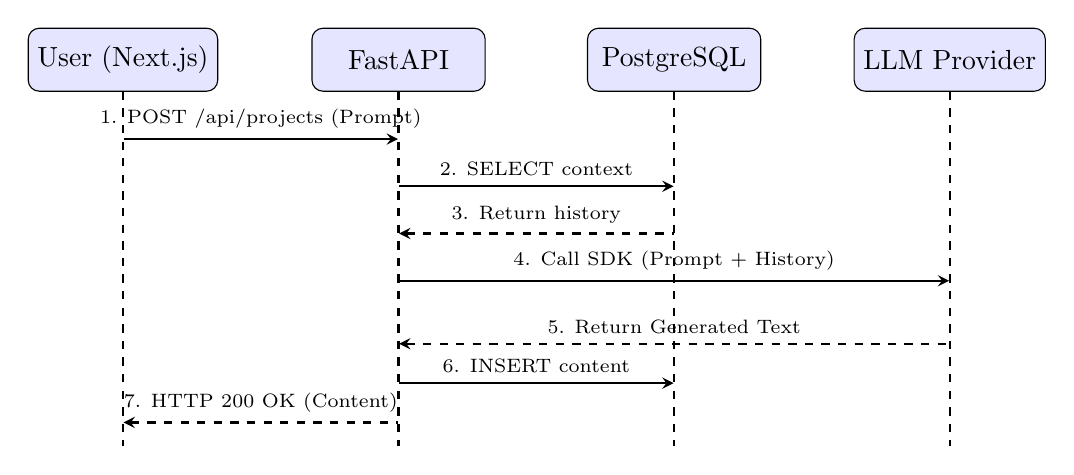
\begin{tikzpicture}[
        node distance=2.5cm,
        auto,
        >=stealth,
        % Định nghĩa style cho các thành phần
        lifeline/.style={thick, dashed},
        % Style cho các "hộp" tên đối tượng
        obj/.style={rectangle, draw, fill=blue!10, text centered, rounded corners, minimum height=0.8cm, minimum width=2.2cm},
        % Style cho điểm neo dọc đường lifeline
        point/.style={circle, inner sep=0pt, minimum size=0pt}
    ]

        % 1. Vẽ các object ở trên cùng
        \node[obj] (user) at (0, 0) {User (Next.js)};
        \node[obj] (api) at (3.5, 0) {FastAPI};
        \node[obj] (db) at (7, 0) {PostgreSQL};
        \node[obj] (llm) at (10.5, 0) {LLM Provider};

        % 2. Vẽ đường lifeline chạy dọc xuống dưới (sử dụng tọa độ tương đối)
        \draw[lifeline] (user.south) -- ++(0,-4.5) node[point] (user_end) {};
        \draw[lifeline] (api.south) -- ++(0,-4.5) node[point] (api_end) {};
        \draw[lifeline] (db.south) -- ++(0,-4.5) node[point] (db_end) {};
        \draw[lifeline] (llm.south) -- ++(0,-4.5) node[point] (llm_end) {};

        % 3. Khai báo các điểm thời gian (Time points) dọc theo các lifeline
        % Điểm thời gian tăng dần từ trên xuống dưới (y âm dần)
        % Mức 1: Tạo request
        \path (user.south) ++(0,-0.6) node[point] (u1) {};
        \path (api.south) ++(0,-0.6) node[point] (a1) {};
        % Mức 2: Lấy history
        \path (api.south) ++(0,-1.2) node[point] (a2) {};
        \path (db.south) ++(0,-1.2) node[point] (d1) {};
        \path (api.south) ++(0,-1.8) node[point] (a3) {};
        \path (db.south) ++(0,-1.8) node[point] (d2) {};
        % Mức 3: Gọi LLM
        \path (api.south) ++(0,-2.4) node[point] (a4) {};
        \path (llm.south) ++(0,-2.4) node[point] (l1) {};
        \path (api.south) ++(0,-3.2) node[point] (a5) {};
        \path (llm.south) ++(0,-3.2) node[point] (l2) {};
        % Mức 4: Ghi DB & Trả kết quả
        \path (api.south) ++(0,-3.7) node[point] (a6) {};
        \path (db.south) ++(0,-3.7) node[point] (d3) {};
        \path (user.south) ++(0,-4.2) node[point] (u2) {};
        \path (api.south) ++(0,-4.2) node[point] (a7) {};

        % 4. Vẽ các mũi tên thông điệp (Messages)
        % User -> API
        \draw[->, thick] (u1) -- node[above, font=\scriptsize] {1. POST /api/projects (Prompt)} (a1);
        % API -> DB
        \draw[->, thick] (a2) -- node[above, font=\scriptsize] {2. SELECT context} (d1);
        \draw[<-, thick, dashed] (a3) -- node[above, font=\scriptsize] {3. Return history} (d2);
        % API -> LLM
        \draw[->, thick] (a4) -- node[above, font=\scriptsize] {4. Call SDK (Prompt + History)} (l1);
        \draw[<-, thick, dashed] (a5) -- node[above, font=\scriptsize] {5. Return Generated Text} (l2);
        % API -> DB
        \draw[->, thick] (a6) -- node[above, font=\scriptsize] {6. INSERT content} (d3);
        % API -> User
        \draw[<-, thick, dashed] (u2) -- node[above, font=\scriptsize] {7. HTTP 200 OK (Content)} (a7);

    \end{tikzpicture}
    \caption{Sơ đồ tuần tự (Sequence Diagram) xử lý tự động sinh nội dung AI}
\end{figure}

\section{Thiết kế Cơ sở dữ liệu}
Mô hình dữ liệu quan hệ được triển khai linh hoạt thông qua PostgreSQL với thiết kế tinh gọn cho giai đoạn đầu, xoay quanh 2 bảng chính có mối quan hệ 1-N. Mọi tương tác của user đều tạo ra dữ liệu gắn chặt vào `Projects`:

\begin{figure}[H]
    \centering
    \begin{tikzpicture}[
        node distance=3cm and 5cm,
        table/.style={
            rectangle, draw, rounded corners=1mm, fill=white,
            align=left, font=\small, inner sep=0pt, minimum width=4cm
        },
        header/.style={
            rectangle, fill=wordblue!80, text=white, font=\bfseries\small, text centered, minimum width=4.5cm, minimum height=0.6cm
        },
        attr/.style={
            font=\small, align=left
        },
        rel/.style={
            diamond, draw, fill=yellow!20, text centered, aspect=2, minimum width=2.5cm, minimum height=1cm
        }
    ]

    % Table Users
    \node[table] (users) at (0, 0) {
        \begin{tabular}{ll}
            \multicolumn{2}{c}{\cellcolor{wordblue!80}\textcolor{white}{\textbf{Users}}} \\ \hline
            \textbf{id} & \textit{UUID (PK)} \\
            email & \textit{String (Unique)} \\
            password\_hash & \textit{String} \\
            created\_at & \textit{Timestamp}
        \end{tabular}
    };

    % Relation 1-N
    \node[rel] (has) at (4.5, 0) {Sở hữu};

    % Table Projects
    \node[table] (projects) at (9, 0) {
        \begin{tabular}{ll}
            \multicolumn{2}{c}{\cellcolor{wordblue!80}\textcolor{white}{\textbf{Projects}}} \\ \hline
            \textbf{id} & \textit{UUID (PK)} \\
            \textbf{user\_id} & \textit{UUID (FK)} \\
            title & \textit{String} \\
            prompt & \textit{Text} \\
            content & \textit{Text} \\
            created\_at & \textit{Timestamp} \\
            updated\_at & \textit{Timestamp}
        \end{tabular}
    };

    % Connecting lines with multiplicity annotations
    \draw[-, thick] (users.east) -- node[above] {1} (has.west);
    \draw[-, thick] (has.east) -- node[above] {N} (projects.west);

    \end{tikzpicture}
    \caption{Lược đồ quan hệ thực thể (ERD) pha MVP 1}
    \label{fig:erd_mvp}
\end{figure}

Lược đồ trên chỉ ra các ràng buộc khóa (Keys constraints) cơ bản của hệ thống:
\begin{itemize}
    \item \textbf{Bảng \texttt{Users}}: Quản lý định danh hệ thống, với khoá chính (\texttt{PK - Primary Key}) là cột \texttt{id}. Cột email phải là duy nhất.
    \item \textbf{Bảng \texttt{Projects}}: 
    \begin{itemize}
        \item Khóa chính (\texttt{PK}) là \texttt{id}, quản lý từng project hoàn toàn phân biệt.
        \item Khóa ngoại (\texttt{FK - Foreign Key}) là \texttt{user\_id}, tham chiếu trực tiếp đến \texttt{Users.id}. Ràng buộc này đảm bảo mối quan hệ \textbf{Một-Nhiều (1-N)} - một người dùng có thể tạo và sở hữu nhiều dự án sáng tạo nội dung, nhưng mỗi dự án chỉ thuộc bản quyền độc lập của nhóm duy nhất người tạo ra (Chặn lỗi truy cập trái phép).
        \item Trường \texttt{prompt} \texttt{content} lưu yêu cầu AI và kết quả sinh (thay thế cho 1 database có bảng chương riêng \texttt{Chapters} trong bản MVP tinh gọn).
    \end{itemize}
\end{itemize}

\chapter{Triển khai hệ thống}
\section{Lựa chọn công nghệ}
% Liệt kê các công nghệ, ưu điểm và lí do lựa chọn so với các lựa chọn khác trên thị trường
Nhóm lựa chọn phân giải hệ thống theo kiến trúc 3 thành phần chính dựa trên ưu điểm vượt trội thực tiễn:
\begin{itemize}
    \item \textbf{Frontend: Next.js (App Router) + TailwindCSS:} Khả năng Server-Side Rendering (SSR) giúp SEO tốt (điều mà React thuần khó làm). Định tuyến App Router mới hỗ trợ tích hợp Layout bảo mật (Protected Routes) rất tối ưu. Tailwind đẩy nhanh vận tốc code giao diện thay vì CSS thuần.
    \item \textbf{Backend: FastAPI (Python):} Đây là công nghệ sinh ra để xử lý các mô hình AI. Đặc điểm I/O Bất đồng bộ (Async) giúp server không bị tắt nghẽn khi phải đợi phản hồi từ OpenAI/Anthropic tính bằng chục giây. Đi kèm `Pydantic` giúp validation API cực kỳ an toàn.
    \item \textbf{Cơ sở dữ liệu - PostgreSQL (Supabase):} Trái với MongoDB, bảng quan hệ (RDBMS) đặc biệt phù hợp để gắn chặt dữ liệu dự án (`Projects`) với Người dùng (`Users`), giúp quản trị phân quyền dễ hơn. Supabase cung cấp nền tảng mã nguồn mở thân thiện cho DevOps.
\end{itemize}

\section{Giai đoạn 1: Minimum Viable Product}
% Phân tích các giao diện cơ bản cần có, thể hiện được tính cơ sở của đồ án, demo thành công tạo novel bằng AI nhằm chứng minh tính khả thi, chưa cần phải giữ ngữ cảnh hoàn toàn.
Trong giai đoạn MVP 1 (Minimum Viable Product), trọng tâm được đặt vào việc kiểm chứng luồng dữ liệu cốt lõi (Core Logic Pipeline), chứng minh hệ thống Backend FastAPI có thể giao tiếp với AI và lưu lại được thành quả xuống DB.

\textbf{Quy trình giao diện cơ bản ở bản Demo 1:}
\begin{enumerate}
    \item \textbf{Đăng nhập/Đăng ký:} Giao diện Auth chuẩn mực, lấy Token JWT và kích hoạt phiên làm việc cá nhân hóa.
    \item \textbf{Bảng điều khiển (Dashboard):} Giao diện truy vấn toàn bộ Project tĩnh (lấy ra từ Postgres) của đúng người dùng đang truy cập.
    \item \textbf{Trình soạn thảo (Workspace):} Nơi người dùng điền "Tiêu đề" và "Prompt" $\rightarrow$ Click [Generate] $\rightarrow$ Backend sẽ chèn dữ liệu vào model, gọi API chờ trả văn bản tiểu thuyết/kịch bản. Văn bản sau khi render sẽ nằm lại vĩnh viễn trong CSDL.
\end{enumerate}

\textbf{Sơ đồ Workflow xử lý MVP (Đăng nhập đến khi nhận kết quả Truyện/Kịch bản):}
\begin{figure}[H]
    \centering
    \begin{tikzpicture}[
        node distance=1.5cm and 1cm,
        auto,
        >=stealth,
        % Style cho các hình khối
        roundrect/.style={rectangle, draw, rounded corners=2mm, fill=blue!10, text centered, align=center, minimum height=0.8cm, minimum width=2.5cm},
        decision/.style={diamond, aspect=2, draw, fill=yellow!10, text centered, align=center, inner sep=0pt, minimum width=2cm, minimum height=1.2cm},
        process/.style={rectangle, draw, fill=green!10, text centered, align=center, minimum height=0.8cm, minimum width=2.5cm},
        dbnode/.style={rectangle, draw, fill=codegreen!20, text centered, align=center, minimum height=0.8cm, minimum width=2cm},
        ai/.style={rectangle, draw, fill=codepurple!20, text centered, align=center, rounded corners=2mm, minimum height=0.8cm, minimum width=2cm}
    ]

        % Vẽ Nodes
        \node[roundrect] (start) at (0, 0) {Trang Đăng Nhập};
        \node[decision] (auth) at (4, 0) {Xác thực \\ (JWT)};
        \node[roundrect] (dash) at (8, 0) {Dashboard \\ (D/s Dự án)};
        
        \node[roundrect] (create) at (8, -2) {Tạo Dự án Mới \\ (Nhập Prompt)};
        \node[process] (api) at (8, -4) {Gửi POST API \\ đến Backend};
        \node[ai] (llm) at (4, -4) {Gọi LLM API \\ (Sinh nội dung)};
        \node[dbnode] (db) at (4, -6) {Lưu trữ DB \\ (PostgreSQL)};
        \node[process] (show) at (8, -6) {Hiển thị Nội dung \\ (Thành công)};

        % Mũi tên
        \draw[->, thick] (start) -- (auth);
        \draw[->, thick] (auth) -- node[above, font=\footnotesize] {Hợp lệ} (dash);
        \draw[->, thick] (dash) -- (create);
        \draw[->, thick] (create) -- (api);
        
        % Chuyển từ API sang LLM và quay lại
        \draw[->, thick] (api) -- node[above, font=\footnotesize] {Prompt} (llm);
        \draw[->, thick] (llm) -- node[right, font=\footnotesize] {Kết quả Text} (db);
        \draw[->, thick] (db) -- node[above, font=\footnotesize] {Phản hồi API} (show);
        
        % Vòng lặp báo lỗi auth
        \draw[->, thick] (auth.south) -- ++(0,-0.8) -| node[pos=0.25, below, font=\footnotesize] {Sai Pass} (start.south);

    \end{tikzpicture}
    \caption{Workflow luồng xử lý chính của MVP 1}
    \label{fig:mvp_workflow}
\end{figure}

MVP 1 tập trung chứng minh tính \textit{Khả thi và Bền Vững của dữ liệu}. Sinh thành công novel 1 lần và bảo vệ cấu trúc CSDL hoàn chỉnh sẽ là bước đệm tuyệt vời để ở các bản sau mở rộng khả năng duy trì Context (Sử dụng Summarize bot) hoàn thiện theo đồ án.


\chapter{Kết luận}
Triển khai hệ thống AI Content Generator đã thành công hoàn thiện toàn bộ bộ khung Client-Server phức tạp với chu trình truyền dữ liệu ổn định, sử dụng Next.js làm giao diện và FastAPI làm luồng lõi kết nối AI. Ở mức MVP 1, hệ thống hoàn toàn đảm bảo khả năng liên kết CSDL PostgreSQL, tiếp nhận prompt người dùng và lưu trữ bản nháp đầu tiên. Lộ trình của dự án rất rõ ràng với lợi thế cạnh tranh về Context-awareness mạnh mẽ, hứa hẹn mở ra tiềm năng thương mại trong lĩnh vực công cụ hỗ trợ cho nhóm họa sĩ, nhà văn và multimedia creators.


\end{document}